%%%%%%%%%%%%%%%%%%%%%%%%%%%%%%%%%%%%%%%%%%%%%%
\section{FDPS並列版詳細記述}
\label{sec:detail}

\subsection{メモリー管理}
\label{sec:memory_management}

\subsubsection{ReallocatableArrayクラス}

この節では, {\tt ReallocatableArray}クラスの詳細記述を行う. 

{\tt ReallocatableArray}クラスは以下の様に記述される。メンバ{\tt
data\_}はT型の配列で、格納最大要素数を{\tt capacity\_}、実際の要素数を
{\tt size\_}に格納する。

\begin{lstlisting}[caption=DomainInfo]
namespace  ParticleSimulator{
    template<class T>
    class ReallocatableArray{
    public:
        T * data_;
        int size_;
        int capacity_;
        ReallocatableArray();
        ReallocatableArray(int capa);
        ReallocatableArray(int size, const T & val);
        ~ReallocatableArray();
        void reserve(const int n);
        int size() const;
        int capacity() const;
        const T & operator [] (const int i) const;
        T & operator [] (const int i);
        T & front(){ return data_[0]; }
        T & back(){ return data_[size_-1]; }
        T * data(){ return data_; }
        const T * data() const { return data_; }
        void push_back(const T & val);
        void resizeNoInitialize(const int n)
        T * getPointer(const int i=0) const;
        void pushBackNoCheck(const T & val){
        long getMemSize() const;
        void dump(const std::string str="");

        }
    };
}
\end{lstlisting}

コンストラクタは以下の3種類。

\begin{screen}
\begin{verbatim}
ReallocatableArray();
\end{verbatim}
\end{screen}

空のクラスを作成する。{\tt std::vector}と同じ振る舞いをする。

\begin{screen}
\begin{verbatim}
ReallocatableArray(int capa);
\end{verbatim}
\end{screen}

{\tt capacity\_}に引数{\tt capa}を代入する。この際、{\tt size\_}は0であ
る。{\tt std::vector}と振る舞いが異なる。

\begin{screen}
\begin{verbatim}
ReallocatableArray(int size, const T & val)
\end{verbatim}
\end{screen}

以下はデストラクタである。

\begin{screen}
\begin{verbatim}
~ReallocatableArray()
\end{verbatim}
\end{screen}

{\tt data\_}の領域が開放される。


{\tt capacity\_}と{\tt size\_}に引数{\tt size}を代入する。またsize個の
要素を引数{¥tt val}で初期化する。{\tt std::vector}と同じ振る舞いをする。

メソッド{\tt reserve()},{\tt size()},{\tt capacity()},{\tt
front()},{\tt back()},{\tt data()},{\tt push\_back()},演算子{\tt []}は
std::vectorのそれとほぼ同じである。

以下には、{\tt AllocatableArray}クラス特有のメソッドを記述する。

\begin{screen}
\begin{verbatim}
public:
void PS::AllocatableArray::resizeNoinitialize(const int n);
\end{verbatim}
\end{screen}

{\tt size\_}に引数{\tt n}を代入する。nが{\tt capacity\_}を超えた場合は
{\tt capacity\_}をnの2倍に変更する。{std::vector::resize}との違いは付け
加えた要素の初期化はされない。


\begin{screen}
\begin{verbatim}
public:
void PS::AllocatableArray::puchBackNoCheck(const T & val);
\end{verbatim}
\end{screen}

{\tt val}を{\tt data\_}の末尾に付け加え、{\tt size\_}を一つインクリメン
トする。{\tt std::vector::push\_back}と違い、配列の領域({\tt
capacity\_})のチェックを行わない。

\begin{screen}
\begin{verbatim}
public:
T * PS::AllocatableArray::getPointer(const int i=0);
\end{verbatim}
\end{screen}
メンバ{\tt data\_}のi番目のポインタを返す。

\begin{screen}
\begin{verbatim}
public:
long getMemSize();
\end{verbatim}
\end{screen}
{\tt data\_}が使用しているバイト数を返す。

\begin{screen}
\begin{verbatim}
public:
void dump(const std::string str="");
\end{verbatim}
\end{screen}

標準出力に引数{\tt str},{\tt size\_},{\tt capacity\_}を表示する。


\subsection{時間計測}
\label{sec:memory_management}

FDPSでは簡易的な時間計測クラス({\tt Timer})を用意した。

{\tt Timer}クラスは以下のように記述されている。

\begin{lstlisting}[caption=Timer]
namespace ParticleSimulator{
    class Timer{
    private:
        enum{
            SPLIT_CAPACITY = 128,
            STRING_SIZE = 1024,
        };
        double begin_time_;
        double end_time_;
        double split_time_[SPLIT_CAPACITY];
        char func_name_[SPLIT_CAPACITY][STRING_SIZE];
        size_t cnt_;
    public:
        void reset();
        void start();
        void stop(const char * str='\0');
        void restart(const char * str='\0');
        void dump(std::ostream & fout);
    };
}
\end{lstlisting}

メソッド、{\tt reset}でクラスの初期化を行い、{\tt start}で現在の時刻を
メンバ{\tt begin\_time\_}に入れる。{\tt stop}で時間計測を止め、現在時
刻と{\tt begin\_time\_}との差をメンバ{\tt split\_time\_[cnt\_]}に格納
する。続けて測定を行いたいときは{\tt stop}ではなく{\tt restart}を使う。
この関数はそこまでの時間を計測し、{\tt split\_time\_[cnt\_]}にその値を
入れる。{\tt restart}するたびにカウンター変数{\tt cnt\_}はインクリメン
トされる。{\tt dump}は全スプリットタイムや最もそのスプリットタイムのか
かったプロセスのランクとその時間を引数{\tt fout}に表示する。

{\tt stop}や{\tt restart}にある引数でそのスプリットタイムを識別するた
めの文字列をメンバ{\tt func\_name\_}入れる事が出来る。この名前は{\tt
dump}を行った時に出力される。


\subsection{標準モジュール詳細}
\label{sec:detail_module}

この節では, 4つのモジュール, すなわち通信用データクラス,領域クラス, 粒
子群クラス, 相互作用ツリークラスの動作の詳細、実装方法を記述する。様々
なデータ構造が現れるが, 断らないかぎり, そのデータ構造はそのクラスに属
す.

%%%%%%%%%%%%%%%%%%%%%%%%%%%%%%%%%%%%%%%%%%%%%%
\subsubsection{通信用データクラス}
\label{sec:detail_module_comm}

\subsubsubsection{}


%\subsubsection{通信用データクラス}
%\label{sec:detail_module_comm}

%%%%%%%%%%%%%%%%%%%%%%%%%%%%%%%%%%%%%%%%%%%%%%
%%\subsubsection{領域クラス}
\label{sec:detail_module_domain_info}

この節では, 領域クラスの詳細記述を行う. 領域クラスの動作は, 初期化, ルー
トドメインの分割である.

領域クラスは以下の様に記述されている。\redtext{このクラスはグローバルに
すべきか?}
\begin{lstlisting}[caption=DomainInfo]
    class DomainInfo{
    private:
        F32vec * pos_sample_tot_;
        F32vec * pos_sample_loc_;
        F32ort * pos_domain_;
        F32ort * pos_domain_temp_;
        F32 coef_ema_;
        S32 target_number_of_sample_particle_;
        S32 number_of_sample_particle_tot_;
        S32 number_of_sample_particle_loc_;
        S32 n_domain_[DIMENSION];
        F32ort pos_root_domain_;
        bool first_call_by_initialize;
        bool first_call_by_decomposeDomain;
        S32 boundary_condition_;
        bool periodic_axis_[DIMENSION];
\end{lstlisting}

\subsubsubsection{初期化}

領域クラスの初期化は, 以下の関数を全プロセスで呼び出すことで行われる.
\begin{screen}
\begin{verbatim}
public:
void PS::DomainInfo::initialize(const PS::F32 coefficient_EMA);
\end{verbatim}
\end{screen}

{\tt coefficient\_EMA}は移動平均の係数である. ここでは移動平均の引数が設
定される. 

この関数は必ず呼び出す必要がある.

\subsubsubsection{領域の分割数の設定}

以下の関数を全プロセスで呼びだすことで, x, y, z軸方向の分割数が設定され
る.
\begin{screen}
\begin{verbatim}
public:
void PS::DomainInfo::setDomain(const PS::S32 nx,
                               const PS::S32 ny,
                               const PS::S32 nz);
\end{verbatim}
\end{screen}

{\tt nx}, {\tt ny}, {\tt nz}はそれぞれ, x, y, z軸方向の分割数である.
{\tt nx}, {\tt ny}, {\tt nz}の積はMPIプロセス数でなければならない. 

この関数は呼出さなくてもよい. この場合, {\tt nx}, {\tt ny}, {\tt nz}の
デフォルト値が採用される. デフォルト値は, 以下のようになっている.  3つ
の積がMPIプロセス数であり, かつそれぞれが最も近い値である. 大小関係は,
{\tt nx >= ny >= nz}となっている.

\subsubsubsubsection{境界条件の設定}

境界条件の設定の設定は, 以下の関数を全プロセスで呼び出すことで行われる.
\begin{screen}
\begin{verbatim}
void setBoundaryCondition(enum BOUNDARY_CONDITION bc);
\end{verbatim}
\end{screen}

引数については、仕様書参照。この関数を呼び出すと、境界条件がメンバ{\tt
boundary\_condition\_}に格納される。また、周期境界条件の場合は周期境界
となる軸の{\tt periodic\_axis\_}が{\tt true}となる(開放境界の軸は{\tt
false})。

以下の関数によって境界条件を得る。
\begin{screen}
\begin{verbatim}
S32 getBoundaryCondition();
\end{verbatim}
\end{screen}

\subsubsubsubsection{ルートドメインの設定}

ルートドメインの設定の詳細記述を行う. ここでは, ルートドメインの形が直
方体であるとする. これは, 開放境界条件と周期境界条件の場合にのみ対応で
きる. 将来的には, この節の名前を「開放境界条件と周期境界条件の場合のルー
トドメインの設定」などに変更する必要があるかもしれない.

ルートドメインの設定は, 以下の関数を全プロセスで呼び出すことで行われる.
\begin{screen}
\begin{verbatim}
public:
void PS::DomainInfo::setRootDomain(const PS::F32ort particle_domain[]);
\end{verbatim}
\end{screen}

引数{\tt particle\_domain}は, 直方体を表す変数である. この直方体がルー
トドメインとなる. ルートドメインは, 最小値側で閉境界, 最大値側で開境界
とする. 

この関数は呼出さなくてもよい. この場合, ルートドメインにはデフォルト値
が採用される.  ルートドメインのデフォルト値は, 単精度浮動小数の最大値と
最小値である(それぞれ{\tt std::numeric\_limits<PS::F32>::max()}, {\tt
- std::numeric\_limits<PS::F32>::max()})と与えられる).

\subsubsubsection{ルートドメインの分割}

この節では, ルートドメインの分割の詳細記述を行う. これは, ルートドメイ
ンの設定, サンプル粒子の回収, 分割の実行の順に行われる.

この動作は, ドメインの分割のために参照する粒子の種類が1つの場合, 以下の
関数を呼び出すだけですむ.
\begin{screen}
\begin{verbatim}
public:
void PS::DomainInfo::decomposeDomainAll(not yet defined);
\end{verbatim}
\end{screen}

以下, 続く.

%%\subsubsubsubsection{前提}

%%各プロセスの持つドメインは固有のID番号(id)を持つ. このID番号はMPIのプロ
%%セスのランク番号と一致する. 番号付けのルールはz, y, x(2次元の場合はy,
%%x)の順で付ける. また, 軸方向のID番号(idx, idy, idz)を持つ. ドメイン固有
%%のID番号と, 軸方向のID番号には以下の関係がある.
%%\begin{equation} 
%%id = idx \times ny \times nz + idy \times nz + idz.
%%\end{equation}
%%ここで, nx, ny, nzはx, y, z軸方向の分割数である. MPIプロセスのランク番
%%号と各軸方向のID番号は通信クラスが保持しており, それぞれ関数{\tt
%%Comm::getRank()}と{\tt Comm::getRankXD(const S32 axis)}で取得できる.

\subsubsubsubsection{サンプル粒子の回収}

サンプル粒子の回収について記述する. 

サンプル粒子の回収をするには, 以下の関数を全プロセスで呼び出すだけでよ
い.
\begin{screen}
\begin{verbatim}
public:
void PS::DomainInfo::collectSampleParticle(const PS::ParticleSystem & psys,
                                           const PS::F32 weight=1.0,
                                           const bool clear=true);
\end{verbatim}
\end{screen}

第1引数{\tt psys}は, サンプルの対象となる粒子の粒子群クラスである. 第2
引数{\tt weight}は, 各プロセスでサンプルする粒子のウェイトである. 第3
引数{\tt clear}はすでにサンプルした粒子のデータを消去するかしないかを決
めるものである. {\tt clear}が, {\tt true}ならば消去し, {\tt false}なら
ば消去しない.

この関数の内部では, {\tt psys}からサンプルした粒子の位置座標を, 領域ク
ラスのメンバ変数である{\tt F32vec}型の配列{\tt pos\_sample\_loc\_}に格
納する. 各プロセスでサンプルする粒子の数の決定と, 実際のサンプルはこの
関数が呼び出す関数{\tt PS::ParticleSystem::getSampleParticle}が行う.

第3引数が{\tt true}だった場合は, {\tt pos\_sample\_loc\_}を空にしてから,
上の動作を行う. 第2引数が{\tt false}だった場合は, {\tt
pos\_sample\_loc\_}を空にせずに, 上の動作を行う.

\redtext{サンプル粒子が全粒子のサブセットであることを
   テスト. あと, インデックスの平均が3sigmaくらいに入ってるかどうか}

\subsubsubsubsection{分割の実行}

分割の実行に関する詳細記述を行う. 

分割の実行を行うには, 全プロセスで, 以下の関数を呼び出すだけでよい.
\begin{screen}
\begin{verbatim}
public:
void PS::DomainInfo::decomposeDomain();
\end{verbatim}
\end{screen}

この関数の内部では以下のことを行う. これらはすべてある1つのプロセス(こ
の節ではルートプロセスと呼ぶ)で行う.  行うことは, Orthogonal Multi
Section (Makino 2004)と同じである.

ルートプロセスに全プロセスから配列{\tt pos\_sample\_loc\_}を集め, 配列
{\tt pos\_sample\_tot\_}に格納する. 

この配列{\tt pos\_sample\_tot\_} を使ってルートドメインを分割する. まず,
ルートドメインをx軸方向に{\tt nx}個のスラブに分割する.  次にこのスラブ
それぞれをy軸方向に{\tt ny}個のカラムに分割する. 最後にこのカラムそれぞ
れをz軸方向に{\tt nz}個のドメインに分割する. これらのドメインの境界を配
列{\tt pos\_domain\_temp\_}に格納する.

配列{\tt pos\_domain\_temp\_}, 配列{\tt pos\_domain\_}, 変数{\tt
coefficient\_EMA}を使って, 移動平均を取り, ドメインの境界を確定する.
この確定したドメインの境界を配列{\tt pos\_domain\_}に格納する. ルート
プロセスは, 配列{\tt pos\_domain\_}を全プロセスに放送する.

\redtext{decomposeDomain: 分割したあとの粒子の分布がサンプル粒子の数に合ってるかどうか}

%%ドメインを切っていく順番はx方向から切り、y、zと順番に切っ
%%ていく。

%%ルートプロセスの{\tt pos\_sample\_}に全プロセスからのサンプル粒子座標が
%%格納されているとする。まず、x軸座標で粒子のソートを行い、各ドメインのx
%%方向の座標を決める。次に、同じドメインに入る粒子のy軸座標でソートを行い、
%%各ドメインのy座標を決める。同様にz軸方向も行う。こうして決まったドメイ
%%ンの座標の配列{\tt pos\_domain\_}を全プロセルに放送する。x軸方向のドメ
%%インの境界が決定した後、y,z軸のドメイン境界の計算は並列に実行する事も出
%%来る。

%%\paragraph{ルートプロセルに全プロセスの粒子を集めない方法}

%%ルートドメイン分割の計算をルートプロセスに実行させると、一番最初のサン
%%プリングやx軸方向のソートが重いと考えられる。そこで、ルートプロセスに全
%%ての粒子を集めない方法を以下に記述する。ただし、この方法は前回のドメイ
%%ンの情報を使っているので、一番最初から使う事は出来ない。

%%\begin{enumerate} \item ドメインのx座標が同じプロセスで作るy-zスラブ
%%内で粒子のサンプリングを行い、スラブ内のidが一番若いプロセスに集める。
%%ここではこのプロセスをルートプロセスと呼ぶ。\item 前回求めたドメイ
%%ンのx座標のみを考えて、収まるべきルートプロセスに粒子を移動させる。
%%\item ルートプロセスのサンプル粒子数のprefix sumを求めておいて、ド
%%メインの分割点を含むプロセスはその座標を計算し、全てのルートプロセ
%%スに放送する。\item 新しく決まったドメイン境界のx座標を使って粒子を移
%%動させる。\end{enumerate}

%%これ以降は、同様の事をy,z軸方向で行ってもよいし、ルートプロセスのみで
%%y,z方向のドメイン座標を計算してもよい。また、多くの場合、各プロセスが一
%%つのドメイン境界を持つと考えられるので、プロセス内でソートせずに選択し
%%てきた方が良いかもしれない。

\subsubsection{領域クラス}
\label{sec:detail_module_domain_info}

この節では, 領域クラスの詳細記述を行う. 領域クラスの動作は, 初期化, ルー
トドメインの分割である.

領域クラスは以下の様に記述されている。\redtext{このクラスはグローバルに
すべきか?}
\begin{lstlisting}[caption=DomainInfo]
    class DomainInfo{
    private:
        F32vec * pos_sample_tot_;
        F32vec * pos_sample_loc_;
        F32ort * pos_domain_;
        F32ort * pos_domain_temp_;
        F32 coef_ema_;
        S32 target_number_of_sample_particle_;
        S32 number_of_sample_particle_tot_;
        S32 number_of_sample_particle_loc_;
        S32 n_domain_[DIMENSION];
        F32ort pos_root_domain_;
        bool first_call_by_initialize;
        bool first_call_by_decomposeDomain;
        S32 boundary_condition_;
        bool periodic_axis_[DIMENSION];
\end{lstlisting}

\subsubsubsection{初期化}

領域クラスの初期化は, 以下の関数を全プロセスで呼び出すことで行われる.
\begin{screen}
\begin{verbatim}
public:
void PS::DomainInfo::initialize(const PS::F32 coefficient_EMA);
\end{verbatim}
\end{screen}

{\tt coefficient\_EMA}は移動平均の係数である. ここでは移動平均の引数が設
定される. 

この関数は必ず呼び出す必要がある.

\subsubsubsection{領域の分割数の設定}

以下の関数を全プロセスで呼びだすことで, x, y, z軸方向の分割数が設定され
る.
\begin{screen}
\begin{verbatim}
public:
void PS::DomainInfo::setDomain(const PS::S32 nx,
                               const PS::S32 ny,
                               const PS::S32 nz);
\end{verbatim}
\end{screen}

{\tt nx}, {\tt ny}, {\tt nz}はそれぞれ, x, y, z軸方向の分割数である.
{\tt nx}, {\tt ny}, {\tt nz}の積はMPIプロセス数でなければならない. 

この関数は呼出さなくてもよい. この場合, {\tt nx}, {\tt ny}, {\tt nz}の
デフォルト値が採用される. デフォルト値は, 以下のようになっている.  3つ
の積がMPIプロセス数であり, かつそれぞれが最も近い値である. 大小関係は,
{\tt nx >= ny >= nz}となっている.

\subsubsubsubsection{境界条件の設定}

境界条件の設定の設定は, 以下の関数を全プロセスで呼び出すことで行われる.
\begin{screen}
\begin{verbatim}
void setBoundaryCondition(enum BOUNDARY_CONDITION bc);
\end{verbatim}
\end{screen}

引数については、仕様書参照。この関数を呼び出すと、境界条件がメンバ{\tt
boundary\_condition\_}に格納される。また、周期境界条件の場合は周期境界
となる軸の{\tt periodic\_axis\_}が{\tt true}となる(開放境界の軸は{\tt
false})。

以下の関数によって境界条件を得る。
\begin{screen}
\begin{verbatim}
S32 getBoundaryCondition();
\end{verbatim}
\end{screen}

\subsubsubsubsection{ルートドメインの設定}

ルートドメインの設定の詳細記述を行う. ここでは, ルートドメインの形が直
方体であるとする. これは, 開放境界条件と周期境界条件の場合にのみ対応で
きる. 将来的には, この節の名前を「開放境界条件と周期境界条件の場合のルー
トドメインの設定」などに変更する必要があるかもしれない.

ルートドメインの設定は, 以下の関数を全プロセスで呼び出すことで行われる.
\begin{screen}
\begin{verbatim}
public:
void PS::DomainInfo::setRootDomain(const PS::F32ort particle_domain[]);
\end{verbatim}
\end{screen}

引数{\tt particle\_domain}は, 直方体を表す変数である. この直方体がルー
トドメインとなる. ルートドメインは, 最小値側で閉境界, 最大値側で開境界
とする. 

この関数は呼出さなくてもよい. この場合, ルートドメインにはデフォルト値
が採用される.  ルートドメインのデフォルト値は, 単精度浮動小数の最大値と
最小値である(それぞれ{\tt std::numeric\_limits<PS::F32>::max()}, {\tt
- std::numeric\_limits<PS::F32>::max()})と与えられる).

\subsubsubsection{ルートドメインの分割}

この節では, ルートドメインの分割の詳細記述を行う. これは, ルートドメイ
ンの設定, サンプル粒子の回収, 分割の実行の順に行われる.

この動作は, ドメインの分割のために参照する粒子の種類が1つの場合, 以下の
関数を呼び出すだけですむ.
\begin{screen}
\begin{verbatim}
public:
void PS::DomainInfo::decomposeDomainAll(not yet defined);
\end{verbatim}
\end{screen}

以下, 続く.

%%\subsubsubsubsection{前提}

%%各プロセスの持つドメインは固有のID番号(id)を持つ. このID番号はMPIのプロ
%%セスのランク番号と一致する. 番号付けのルールはz, y, x(2次元の場合はy,
%%x)の順で付ける. また, 軸方向のID番号(idx, idy, idz)を持つ. ドメイン固有
%%のID番号と, 軸方向のID番号には以下の関係がある.
%%\begin{equation} 
%%id = idx \times ny \times nz + idy \times nz + idz.
%%\end{equation}
%%ここで, nx, ny, nzはx, y, z軸方向の分割数である. MPIプロセスのランク番
%%号と各軸方向のID番号は通信クラスが保持しており, それぞれ関数{\tt
%%Comm::getRank()}と{\tt Comm::getRankXD(const S32 axis)}で取得できる.

\subsubsubsubsection{サンプル粒子の回収}

サンプル粒子の回収について記述する. 

サンプル粒子の回収をするには, 以下の関数を全プロセスで呼び出すだけでよ
い.
\begin{screen}
\begin{verbatim}
public:
void PS::DomainInfo::collectSampleParticle(const PS::ParticleSystem & psys,
                                           const PS::F32 weight=1.0,
                                           const bool clear=true);
\end{verbatim}
\end{screen}

第1引数{\tt psys}は, サンプルの対象となる粒子の粒子群クラスである. 第2
引数{\tt weight}は, 各プロセスでサンプルする粒子のウェイトである. 第3
引数{\tt clear}はすでにサンプルした粒子のデータを消去するかしないかを決
めるものである. {\tt clear}が, {\tt true}ならば消去し, {\tt false}なら
ば消去しない.

この関数の内部では, {\tt psys}からサンプルした粒子の位置座標を, 領域ク
ラスのメンバ変数である{\tt F32vec}型の配列{\tt pos\_sample\_loc\_}に格
納する. 各プロセスでサンプルする粒子の数の決定と, 実際のサンプルはこの
関数が呼び出す関数{\tt PS::ParticleSystem::getSampleParticle}が行う.

第3引数が{\tt true}だった場合は, {\tt pos\_sample\_loc\_}を空にしてから,
上の動作を行う. 第2引数が{\tt false}だった場合は, {\tt
pos\_sample\_loc\_}を空にせずに, 上の動作を行う.

\redtext{サンプル粒子が全粒子のサブセットであることを
   テスト. あと, インデックスの平均が3sigmaくらいに入ってるかどうか}

\subsubsubsubsection{分割の実行}

分割の実行に関する詳細記述を行う. 

分割の実行を行うには, 全プロセスで, 以下の関数を呼び出すだけでよい.
\begin{screen}
\begin{verbatim}
public:
void PS::DomainInfo::decomposeDomain();
\end{verbatim}
\end{screen}

この関数の内部では以下のことを行う. これらはすべてある1つのプロセス(こ
の節ではルートプロセスと呼ぶ)で行う.  行うことは, Orthogonal Multi
Section (Makino 2004)と同じである.

ルートプロセスに全プロセスから配列{\tt pos\_sample\_loc\_}を集め, 配列
{\tt pos\_sample\_tot\_}に格納する. 

この配列{\tt pos\_sample\_tot\_} を使ってルートドメインを分割する. まず,
ルートドメインをx軸方向に{\tt nx}個のスラブに分割する.  次にこのスラブ
それぞれをy軸方向に{\tt ny}個のカラムに分割する. 最後にこのカラムそれぞ
れをz軸方向に{\tt nz}個のドメインに分割する. これらのドメインの境界を配
列{\tt pos\_domain\_temp\_}に格納する.

配列{\tt pos\_domain\_temp\_}, 配列{\tt pos\_domain\_}, 変数{\tt
coefficient\_EMA}を使って, 移動平均を取り, ドメインの境界を確定する.
この確定したドメインの境界を配列{\tt pos\_domain\_}に格納する. ルート
プロセスは, 配列{\tt pos\_domain\_}を全プロセスに放送する.

\redtext{decomposeDomain: 分割したあとの粒子の分布がサンプル粒子の数に合ってるかどうか}

%%ドメインを切っていく順番はx方向から切り、y、zと順番に切っ
%%ていく。

%%ルートプロセスの{\tt pos\_sample\_}に全プロセスからのサンプル粒子座標が
%%格納されているとする。まず、x軸座標で粒子のソートを行い、各ドメインのx
%%方向の座標を決める。次に、同じドメインに入る粒子のy軸座標でソートを行い、
%%各ドメインのy座標を決める。同様にz軸方向も行う。こうして決まったドメイ
%%ンの座標の配列{\tt pos\_domain\_}を全プロセルに放送する。x軸方向のドメ
%%インの境界が決定した後、y,z軸のドメイン境界の計算は並列に実行する事も出
%%来る。

%%\paragraph{ルートプロセルに全プロセスの粒子を集めない方法}

%%ルートドメイン分割の計算をルートプロセスに実行させると、一番最初のサン
%%プリングやx軸方向のソートが重いと考えられる。そこで、ルートプロセスに全
%%ての粒子を集めない方法を以下に記述する。ただし、この方法は前回のドメイ
%%ンの情報を使っているので、一番最初から使う事は出来ない。

%%\begin{enumerate} \item ドメインのx座標が同じプロセスで作るy-zスラブ
%%内で粒子のサンプリングを行い、スラブ内のidが一番若いプロセスに集める。
%%ここではこのプロセスをルートプロセスと呼ぶ。\item 前回求めたドメイ
%%ンのx座標のみを考えて、収まるべきルートプロセスに粒子を移動させる。
%%\item ルートプロセスのサンプル粒子数のprefix sumを求めておいて、ド
%%メインの分割点を含むプロセスはその座標を計算し、全てのルートプロセ
%%スに放送する。\item 新しく決まったドメイン境界のx座標を使って粒子を移
%%動させる。\end{enumerate}

%%これ以降は、同様の事をy,z軸方向で行ってもよいし、ルートプロセスのみで
%%y,z方向のドメイン座標を計算してもよい。また、多くの場合、各プロセスが一
%%つのドメイン境界を持つと考えられるので、プロセス内でソートせずに選択し
%%てきた方が良いかもしれない。


%\subsubsection{領域クラス}
%\label{sec:detail_module_domain_info}


%%%%%%%%%%%%%%%%%%%%%%%%%%%%%%%%%%%%%%%%%%%%%%
%%\subsubsection{粒子群クラス}
\label{sec:detail_module_paricle_system}

\subsubsubsection{ファイル入力}

ここでは、ユーザーが用意した粒子の初期条件ファイルの入力メソッドについて記述する。

ファイル入力を行う関数は以下の二つである。

\begin{screen}
\begin{verbatim}
void loadParticleSingle(
                        const char * filename,
                        const char * mode,
                        void (*(FullParticle::pfunc))(FILE *));
\end{verbatim}
\end{screen}

\begin{screen}
\begin{verbatim}
void loadParticle(
                  const char * format,
                  const char * mode,
                  void (*(FullParticle::pfunc))(FILE *))
\end{verbatim}
\end{screen}

前者は一つの初期条件ファイルを読み込む場合、後者はファイルが分割されて
いる場合に使う。

これらの関数では、以下の様にメンバが設定、変更される。
\begin{itemize}
\item プロセスの持つ粒子数{\tt n\_ptcl\_loc\_}を設定。
\item 全プロセスが持つ粒子数の合計{\tt n\_ptcl\_tot\_}を設定。
\item {\tt ptcl\_}の配列サイズ{\tt n\_ptcl\_loc\_max\_}を設定。
\item {\tt ptcl\_}の配列の確保と初期条件ファイルからの代入。
\end{itemize}


まず、{\tt loadParticleSingle(...)}。大まかな流れはプロセス番号0のプロ
セスがユーザーが用意した初期条件ファイルからユーザーが定義した粒子読み
取り関数(フルパーティクルクラスのメソッド)を使って粒子データを読み取
り、各プロセスの持つ粒子数が同じになるようにフルパーティクルデータを送
信する。ユーザーが用意する初期条件ファイルはアスキーの場合は一行に一粒
子の情報が書き込まれていなければならない。バイナリーの場合は一粒子ごと
まとまって情報が書かれている必要がある。アスキー、バイナリーは第二引数
で{\tt "r"}、{\tt "rb"}を選択する事で切り替える。これら以外のものが設定
された場合は例外を送出する。粒子読み取り関数は以下の様に定義されている。

\begin{verbatim}
void FullParticle::loadOneParticleAscDec(FILE *fp) {
    fscanf(fp, "%lf%lf%lf%lf%lf%lf%lf",
                  &this->mass,
                  &this->pos[0], &this->pos[1], &this->pos[2],
                  &this->vel[0], &this->vel[1], &this->vel[2]);
}
\end{verbatim}

初期条件ファイルには、粒子数の情報が無いので、最初にファイルを終りまで
読み込み粒子数を数え、それをメンバ{\tt n\_ptcl\_tot\_}に格納し、{\tt
n\_ptcl\_tot\_}とプロセス数から、各プロセスが持つ粒子数{\tt
n\_ptcl\_loc\_}と{\tt ptcl\_}の配列の大きさ{\tt n\_ptcl\_loc\_max\_}を
決定し、{\tt ptcl\_}の配列を確保する。

{\tt n\_ptcl\_loc\_max\_}はデフォルトでは以下の様に決定する。

\begin{equation}
{\rm n\_ptcl\_loc\_max\_} = {\rm n\_ptcl\_tot\_} / プロセス数 * 4 + 1000;
\end{equation}

配列の大きさの決め方はユーザーも定義出来るようにしたいが、どの様にする
かは決まっていない。

{\tt n\_ptcl\_loc\_}は各プロセスで同じになるようにする。{\tt
n\_ptcl\_tot\_}がプロセス数で割り切れない場合はプロセス番号の若いプロセ
スから順に粒子を一つ多く持つようにする。ここまで実行したのち、再びファ
イルを頭から読み込み、データを{\tt ptcl\_}に格納する。

次に、{\tt loadParticle(...)}の詳細について述べる。ユーザーが用意する粒
子の初期条件ファイルの形式や読み込み関数は{\tt loadParticleSingl(...)}
の場合と同じである。第一引数{\tt fileformat}でファイル名のフォーマット
を指定する。フォーマットの指定方法は標準Cライブラリの関数\verb|printf|
の第1引数と同じである。ただし変換指定は必ず2つであり、その指定子はどち
らも整数である。1つ目の変換指定にはそのジョブの全プロセス数が、2つ目の
変換指定にはプロセス番号が入る。例えば、引数が
\verb|nbody_%03d_%03d.init|ならば、全プロセス数$64$のジョブのプロセス番
号$12$のプロセスは、\verb|nbody_064_012.init|というファイルを読み込む。
フォーマットの指定正しくない場合は例外を送出する。

各プロセスは割り当てられた初期条件ファイルから粒子データを読み取り{\tt
ptcl\_}に格納する。初期条件ファイルには、粒子数の情報が無いので、最初に
ファイルを終りまで読み込み粒子数を数え、それをメンバ{\tt
n\_ptcl\_loc\_}に格納し、{\tt MPI::Allreduce}を使って{\tt
n\_ptcl\_loc\_}の和を{\tt n\_ptcl\_tot\_}に格納する。{\tt
n\_ptcl\_tot\_}とプロセス数から、{\tt ptcl\_}の配列の大きさ{\tt
n\_ptcl\_loc\_max\_}を{\tt loadParticleSingle(...)}の場合と同じ方法で決
定し、{ptcl\_}の配列を確保する。もし、{\tt n\_ptcl\_loc\_max\_}が{\tt
n\_ptcl\_loc\_}より、小さくなってしまった場合は例外を送出する。

\subsubsubsection{ファイル出力}

%ここでは、ユーザーが用意した粒子のスナップショットファイルの出力メソッ
%ドについて記述する。

%ファイル出力を行う関数は以下の二つである。

%\begin{screen}
%\begin{verbatim}
%void PS::ParticleSystem::dumpParticleSingle(
%                            const char * filename,
%                            const char * mode,
%                            void (*(FullParticle::pfunc))(FILE *))
%\end{verbatim}
%\end{screen}

%\begin{screen}
%\begin{verbatim}
%void PS::ParticleSystem::dumpParticle(
%                            const char * format,
%                            const char * mode,
%                            void (*(FullParticle::pfunc))(FILE *))
%\end{verbatim}
%\end{screen}

%前者は一つのスナップショットファイルを出力する場合、後者は各プロセスが
%ファイルを出力する場合に使う。

%まず、前者について述べる。大まかな流れは、以下の様である。プロセス番号
%iのプロセスがユーザーの定義した一粒子書き込み関数にしたがって、{\tt
%ptcl_}から情報をダンプし、そのプロセスの持つ全ての粒子をダンプしたら、
%ファイルポインタをプロセス番号i+1のプロセスに渡し、同様に粒子データをダ
%ンプする。

%{\tt mode}は以下の四つが定義されている。
%\begin{tabular}{llll} 
%{\tt mode} &=& {\tt "w"} & アスキー用 \\ 
%     &=& {\tt "wb"} & バイナリー用 \\
%     &=& {\tt "a"} & 追加書き込みアスキー用 \\
%     &=& {\tt "ab"} & 追加書き込みバイナリー用
%\end{tabular}
%これ以外が選ばれた場合は例外を送出する。

%また、一粒子書き込み関数は以下の様に定義してもらう。
%\begin{verbatim}
%void RealParticle::dumpOneParticleAscDec(FILE *fp) {
%    fprintf(fp, "%lf %lf %lf %lf %lf %lf %lf %lf %lf %lf\n",
%                   this->mass,
%                   this->pos[0], this->pos[1], this->pos[2],
%                   this->vel[0], this->vel[1], this->vel[2],
%                   this->acc[0], this->acc[1], this->acc[2]);
%}
%\end{verbatim}

\subsubsubsection{初期設定}

\begin{screen}
\begin{verbatim}
public:
void PS::ParticleSystem::initialize()
\end{verbatim}
\end{screen}

いまのところやることがないが, そのうちできるかもしれないので, とりあえ
ず残しておく.

\subsubsubsection{粒子配列のメモリ確保}

各プロセスにおける粒子配列のメモリ確保は, 以下の関数を各プロセスで呼び
出すことで行われる.
\begin{screen}
\begin{verbatim}
public:
void PS::ParticleSystem::createParticle(const PS::S32 n_limit)
\end{verbatim}
\end{screen}

引数{\tt n\_limit}は粒子配列のサイズである. 

この関数は必ず呼出されなければならない.

\subsubsubsection{サンプル粒子数の設定}

\begin{screen}
\begin{verbatim}
public:
void PS::ParticleSystem::setAvarageTargetNumberOfSampleParticlePerProcess
(const PS::S32 nsampleperprocess)
\end{verbatim}
\end{screen}

引数は, 領域分割のためにサンプルする粒子の目標数. この目標数は, 各プロ
セスがある粒子種で集める粒子数の平均である. この粒子数と全プロセス数か
ら, 全プロセスでサンプルすべき粒子数を求めることができ, この数が{\tt
n\_smp\_ptcl\_tot\_}に格納される.

この関数は呼出さなくてもよい. この場合, デフォルト値が採用される. デフォ
ルト値は30である.

%%\subsubsubsection{あるプロセスの担当する粒子を包含する最小の直方体を求める関数}
%%
%%あるプロセスの担当するある粒子種すべてを包含する最小の直方体を求める関
%%数である.
%%\begin{screen}
%%\begin{verbatim}
%%public:
%%PS::F32ort PS::ParticleSystem::getParticleDomain(void)
%%\end{verbatim}
%%\end{screen}
%%この直方体は, この関数を呼ぶと, 返値としてあたえられる.
%%
%%内部で行っていることは, ある粒子種の各軸方向の最大値最小値を取るだけである.

\subsubsubsection{リアル粒子のサンプル}

各プロセスで以下の関数を呼び出すと, 各プロセスでその担当粒子から粒子の
サンプルが行われる.
\begin{screen}
\begin{verbatim}
public:
void PS::ParticleSystem::getSampleParticle(PS::S32 & number_of_sample_particle,
                                           PS::F32vec pos_sample [],
                                           const PS::F32 weight)
\end{verbatim}
\end{screen}

第1, 第2引数は出力である. 第1引数{\tt number\_of\_sample\_partile}はサ
ンプルする粒子の数, 第2引数{\tt pos\_sample}はサンプルした粒子の位置座
標である. 第3引数は入力であり, そのプロセスでサンプルすべき粒子の数のウェ
イトである.

サンプルする粒子の数は{\tt (PS::S32) (weight * n\_smp\_ptcl\_tot\_ /
weight\_all)}として与えられる. {\tt weight\_all}は全プロセスの{\tt
weight}の和である.

サンプルする粒子はメルセンヌ・ツイスター法を用いたモンテカルロ法で選ば
れる.

この関数は領域クラスのメンバ関数である{\tt collectSampleParticle}で呼出
されるだけであり, ユーザーに使用されることはない.

\redtext{getSampleParticle: テストDomainInfo::collectSampleParticleと同じような感じ}

\subsubsubsection{リアル粒子の交換}

この節では, リアル粒子の交換に関する詳細記述を行う. この動作は以下の関
数を全プロセスで呼び出すことで行われる.
\begin{screen}
\begin{verbatim}
public:
void PS::ParticleSystem::exchangeParticle(const PS::DomainInfo & dinfo)
\end{verbatim}
\end{screen}

%%この関数では、以下の様にメンバが設定、変更される。
%%\begin{itemize}
%%\item 他プロセスからの粒子を{\tt ptcl\_}に格納する。
%%\item {\tt n\_ptcl\_loc\_}を設定。
%%\end{itemize}

手順は以下の2段階. 1段階目では, 領域クラスのメンバ変数で{\tt
PS::F32ort}型の配列{\tt pos\_domain\_}を使って, 各粒子がどのドメインに
入るかを計算する. 2段目では, 自プロセス以外が担当するドメインに入る粒子
があれば, フルパーティクルデータごと該当プロセスへ送信する.

%%1段階目を記述する. 各プロセスは, 各粒子に対して, どのドメインに入るかを
%%決める. (以下書きかけ) どのドメインに入るかはツリー構造を使って探す. 送
%%信バッファは前回のサイズから推定, リンクトリストの使用, またはループを
%%2回まわすことで設定する.

1段階目を記述する. これは各プロセスで行われる. 行われることは以下の通り.
各粒子に対して, 自分のドメインに入るか, 入らないかを調べる. もし入らな
い場合, その粒子が入るドメインを探す. 探し方は以下の通り. まず, その粒
子が入るスラブを探す. 次に, その粒子が, そのスラブ内のどのカラムに入る
かを探す. 最後に, その粒子が, そのカラム内のどのドメインに入るかを探す.
上記のスラブ, カラム, ドメインの探し方は, 二分探索である.

%%2段階目を記述する. 各プロセスは, 他のプロセスにフルパーティクルデータを
%%送る. (以下書きかけ) {\tt ptcl\_}には, 元々自プロセスが持っていた粒子が
%%先頭, 他プロセスから送られてきた粒子は後に置くことにする.

2段階目を記述する. 各プロセスは, 他のプロセスにフルパーティクルデータを
送る. {\tt ptcl\_}には, 元々自プロセスが持っていた粒子が先頭, 他プロセ
スから送られてきた粒子は後に置くことにする.

%%実装方法は大きく2通り考えられる。一つはプロセス数でループを回し、さら
%%に粒子方向にもループを回して、粒子の行き先のプロセスを探して、送信バッ
%%ファに入れていく方法。もう一つは粒子方向でループを回し、各粒子がどの
%%プロセスに行くかを探す方法である。

%%後者では粒子の行き先を探すのにルートドメインの分割のツリー構造が使え
%%るため、高速であるが、各送信バッファに入る粒子数は最後までわからない。
%%しかし、送信バッファのサイズは前回のサイズから推定する事も出来るし、
%%そうでなくてもリンクトリストを使ったり、ループを二回回して、最初のルー
%%プで送信する粒子の個数を数えて、2回目で粒子を送信用バッファーにコピー
%%すればよい。なので、後者の方法を採用する。

%%この関数を呼んだ後には、{\tt ptcl\_}には新たな粒子が設定されている。
%%粒子の並びは先頭が元々自プロセルが持っていた粒子で、その後ろに他プロ
%%セスから来た粒子が並ぶようにする。

\subsubsection{粒子群クラス}
\label{sec:detail_module_paricle_system}

\subsubsubsection{ファイル入力}

ここでは、ユーザーが用意した粒子の初期条件ファイルの入力メソッドについて記述する。

ファイル入力を行う関数は以下の二つである。

\begin{screen}
\begin{verbatim}
void loadParticleSingle(
                        const char * filename,
                        const char * mode,
                        void (*(FullParticle::pfunc))(FILE *));
\end{verbatim}
\end{screen}

\begin{screen}
\begin{verbatim}
void loadParticle(
                  const char * format,
                  const char * mode,
                  void (*(FullParticle::pfunc))(FILE *))
\end{verbatim}
\end{screen}

前者は一つの初期条件ファイルを読み込む場合、後者はファイルが分割されて
いる場合に使う。

これらの関数では、以下の様にメンバが設定、変更される。
\begin{itemize}
\item プロセスの持つ粒子数{\tt n\_ptcl\_loc\_}を設定。
\item 全プロセスが持つ粒子数の合計{\tt n\_ptcl\_tot\_}を設定。
\item {\tt ptcl\_}の配列サイズ{\tt n\_ptcl\_loc\_max\_}を設定。
\item {\tt ptcl\_}の配列の確保と初期条件ファイルからの代入。
\end{itemize}


まず、{\tt loadParticleSingle(...)}。大まかな流れはプロセス番号0のプロ
セスがユーザーが用意した初期条件ファイルからユーザーが定義した粒子読み
取り関数(フルパーティクルクラスのメソッド)を使って粒子データを読み取
り、各プロセスの持つ粒子数が同じになるようにフルパーティクルデータを送
信する。ユーザーが用意する初期条件ファイルはアスキーの場合は一行に一粒
子の情報が書き込まれていなければならない。バイナリーの場合は一粒子ごと
まとまって情報が書かれている必要がある。アスキー、バイナリーは第二引数
で{\tt "r"}、{\tt "rb"}を選択する事で切り替える。これら以外のものが設定
された場合は例外を送出する。粒子読み取り関数は以下の様に定義されている。

\begin{verbatim}
void FullParticle::loadOneParticleAscDec(FILE *fp) {
    fscanf(fp, "%lf%lf%lf%lf%lf%lf%lf",
                  &this->mass,
                  &this->pos[0], &this->pos[1], &this->pos[2],
                  &this->vel[0], &this->vel[1], &this->vel[2]);
}
\end{verbatim}

初期条件ファイルには、粒子数の情報が無いので、最初にファイルを終りまで
読み込み粒子数を数え、それをメンバ{\tt n\_ptcl\_tot\_}に格納し、{\tt
n\_ptcl\_tot\_}とプロセス数から、各プロセスが持つ粒子数{\tt
n\_ptcl\_loc\_}と{\tt ptcl\_}の配列の大きさ{\tt n\_ptcl\_loc\_max\_}を
決定し、{\tt ptcl\_}の配列を確保する。

{\tt n\_ptcl\_loc\_max\_}はデフォルトでは以下の様に決定する。

\begin{equation}
{\rm n\_ptcl\_loc\_max\_} = {\rm n\_ptcl\_tot\_} / プロセス数 * 4 + 1000;
\end{equation}

配列の大きさの決め方はユーザーも定義出来るようにしたいが、どの様にする
かは決まっていない。

{\tt n\_ptcl\_loc\_}は各プロセスで同じになるようにする。{\tt
n\_ptcl\_tot\_}がプロセス数で割り切れない場合はプロセス番号の若いプロセ
スから順に粒子を一つ多く持つようにする。ここまで実行したのち、再びファ
イルを頭から読み込み、データを{\tt ptcl\_}に格納する。

次に、{\tt loadParticle(...)}の詳細について述べる。ユーザーが用意する粒
子の初期条件ファイルの形式や読み込み関数は{\tt loadParticleSingl(...)}
の場合と同じである。第一引数{\tt fileformat}でファイル名のフォーマット
を指定する。フォーマットの指定方法は標準Cライブラリの関数\verb|printf|
の第1引数と同じである。ただし変換指定は必ず2つであり、その指定子はどち
らも整数である。1つ目の変換指定にはそのジョブの全プロセス数が、2つ目の
変換指定にはプロセス番号が入る。例えば、引数が
\verb|nbody_%03d_%03d.init|ならば、全プロセス数$64$のジョブのプロセス番
号$12$のプロセスは、\verb|nbody_064_012.init|というファイルを読み込む。
フォーマットの指定正しくない場合は例外を送出する。

各プロセスは割り当てられた初期条件ファイルから粒子データを読み取り{\tt
ptcl\_}に格納する。初期条件ファイルには、粒子数の情報が無いので、最初に
ファイルを終りまで読み込み粒子数を数え、それをメンバ{\tt
n\_ptcl\_loc\_}に格納し、{\tt MPI::Allreduce}を使って{\tt
n\_ptcl\_loc\_}の和を{\tt n\_ptcl\_tot\_}に格納する。{\tt
n\_ptcl\_tot\_}とプロセス数から、{\tt ptcl\_}の配列の大きさ{\tt
n\_ptcl\_loc\_max\_}を{\tt loadParticleSingle(...)}の場合と同じ方法で決
定し、{ptcl\_}の配列を確保する。もし、{\tt n\_ptcl\_loc\_max\_}が{\tt
n\_ptcl\_loc\_}より、小さくなってしまった場合は例外を送出する。

\subsubsubsection{ファイル出力}

%ここでは、ユーザーが用意した粒子のスナップショットファイルの出力メソッ
%ドについて記述する。

%ファイル出力を行う関数は以下の二つである。

%\begin{screen}
%\begin{verbatim}
%void PS::ParticleSystem::dumpParticleSingle(
%                            const char * filename,
%                            const char * mode,
%                            void (*(FullParticle::pfunc))(FILE *))
%\end{verbatim}
%\end{screen}

%\begin{screen}
%\begin{verbatim}
%void PS::ParticleSystem::dumpParticle(
%                            const char * format,
%                            const char * mode,
%                            void (*(FullParticle::pfunc))(FILE *))
%\end{verbatim}
%\end{screen}

%前者は一つのスナップショットファイルを出力する場合、後者は各プロセスが
%ファイルを出力する場合に使う。

%まず、前者について述べる。大まかな流れは、以下の様である。プロセス番号
%iのプロセスがユーザーの定義した一粒子書き込み関数にしたがって、{\tt
%ptcl_}から情報をダンプし、そのプロセスの持つ全ての粒子をダンプしたら、
%ファイルポインタをプロセス番号i+1のプロセスに渡し、同様に粒子データをダ
%ンプする。

%{\tt mode}は以下の四つが定義されている。
%\begin{tabular}{llll} 
%{\tt mode} &=& {\tt "w"} & アスキー用 \\ 
%     &=& {\tt "wb"} & バイナリー用 \\
%     &=& {\tt "a"} & 追加書き込みアスキー用 \\
%     &=& {\tt "ab"} & 追加書き込みバイナリー用
%\end{tabular}
%これ以外が選ばれた場合は例外を送出する。

%また、一粒子書き込み関数は以下の様に定義してもらう。
%\begin{verbatim}
%void RealParticle::dumpOneParticleAscDec(FILE *fp) {
%    fprintf(fp, "%lf %lf %lf %lf %lf %lf %lf %lf %lf %lf\n",
%                   this->mass,
%                   this->pos[0], this->pos[1], this->pos[2],
%                   this->vel[0], this->vel[1], this->vel[2],
%                   this->acc[0], this->acc[1], this->acc[2]);
%}
%\end{verbatim}

\subsubsubsection{初期設定}

\begin{screen}
\begin{verbatim}
public:
void PS::ParticleSystem::initialize()
\end{verbatim}
\end{screen}

いまのところやることがないが, そのうちできるかもしれないので, とりあえ
ず残しておく.

\subsubsubsection{粒子配列のメモリ確保}

各プロセスにおける粒子配列のメモリ確保は, 以下の関数を各プロセスで呼び
出すことで行われる.
\begin{screen}
\begin{verbatim}
public:
void PS::ParticleSystem::createParticle(const PS::S32 n_limit)
\end{verbatim}
\end{screen}

引数{\tt n\_limit}は粒子配列のサイズである. 

この関数は必ず呼出されなければならない.

\subsubsubsection{サンプル粒子数の設定}

\begin{screen}
\begin{verbatim}
public:
void PS::ParticleSystem::setAvarageTargetNumberOfSampleParticlePerProcess
(const PS::S32 nsampleperprocess)
\end{verbatim}
\end{screen}

引数は, 領域分割のためにサンプルする粒子の目標数. この目標数は, 各プロ
セスがある粒子種で集める粒子数の平均である. この粒子数と全プロセス数か
ら, 全プロセスでサンプルすべき粒子数を求めることができ, この数が{\tt
n\_smp\_ptcl\_tot\_}に格納される.

この関数は呼出さなくてもよい. この場合, デフォルト値が採用される. デフォ
ルト値は30である.

%%\subsubsubsection{あるプロセスの担当する粒子を包含する最小の直方体を求める関数}
%%
%%あるプロセスの担当するある粒子種すべてを包含する最小の直方体を求める関
%%数である.
%%\begin{screen}
%%\begin{verbatim}
%%public:
%%PS::F32ort PS::ParticleSystem::getParticleDomain(void)
%%\end{verbatim}
%%\end{screen}
%%この直方体は, この関数を呼ぶと, 返値としてあたえられる.
%%
%%内部で行っていることは, ある粒子種の各軸方向の最大値最小値を取るだけである.

\subsubsubsection{リアル粒子のサンプル}

各プロセスで以下の関数を呼び出すと, 各プロセスでその担当粒子から粒子の
サンプルが行われる.
\begin{screen}
\begin{verbatim}
public:
void PS::ParticleSystem::getSampleParticle(PS::S32 & number_of_sample_particle,
                                           PS::F32vec pos_sample [],
                                           const PS::F32 weight)
\end{verbatim}
\end{screen}

第1, 第2引数は出力である. 第1引数{\tt number\_of\_sample\_partile}はサ
ンプルする粒子の数, 第2引数{\tt pos\_sample}はサンプルした粒子の位置座
標である. 第3引数は入力であり, そのプロセスでサンプルすべき粒子の数のウェ
イトである.

サンプルする粒子の数は{\tt (PS::S32) (weight * n\_smp\_ptcl\_tot\_ /
weight\_all)}として与えられる. {\tt weight\_all}は全プロセスの{\tt
weight}の和である.

サンプルする粒子はメルセンヌ・ツイスター法を用いたモンテカルロ法で選ば
れる.

この関数は領域クラスのメンバ関数である{\tt collectSampleParticle}で呼出
されるだけであり, ユーザーに使用されることはない.

\redtext{getSampleParticle: テストDomainInfo::collectSampleParticleと同じような感じ}

\subsubsubsection{リアル粒子の交換}

この節では, リアル粒子の交換に関する詳細記述を行う. この動作は以下の関
数を全プロセスで呼び出すことで行われる.
\begin{screen}
\begin{verbatim}
public:
void PS::ParticleSystem::exchangeParticle(const PS::DomainInfo & dinfo)
\end{verbatim}
\end{screen}

%%この関数では、以下の様にメンバが設定、変更される。
%%\begin{itemize}
%%\item 他プロセスからの粒子を{\tt ptcl\_}に格納する。
%%\item {\tt n\_ptcl\_loc\_}を設定。
%%\end{itemize}

手順は以下の2段階. 1段階目では, 領域クラスのメンバ変数で{\tt
PS::F32ort}型の配列{\tt pos\_domain\_}を使って, 各粒子がどのドメインに
入るかを計算する. 2段目では, 自プロセス以外が担当するドメインに入る粒子
があれば, フルパーティクルデータごと該当プロセスへ送信する.

%%1段階目を記述する. 各プロセスは, 各粒子に対して, どのドメインに入るかを
%%決める. (以下書きかけ) どのドメインに入るかはツリー構造を使って探す. 送
%%信バッファは前回のサイズから推定, リンクトリストの使用, またはループを
%%2回まわすことで設定する.

1段階目を記述する. これは各プロセスで行われる. 行われることは以下の通り.
各粒子に対して, 自分のドメインに入るか, 入らないかを調べる. もし入らな
い場合, その粒子が入るドメインを探す. 探し方は以下の通り. まず, その粒
子が入るスラブを探す. 次に, その粒子が, そのスラブ内のどのカラムに入る
かを探す. 最後に, その粒子が, そのカラム内のどのドメインに入るかを探す.
上記のスラブ, カラム, ドメインの探し方は, 二分探索である.

%%2段階目を記述する. 各プロセスは, 他のプロセスにフルパーティクルデータを
%%送る. (以下書きかけ) {\tt ptcl\_}には, 元々自プロセスが持っていた粒子が
%%先頭, 他プロセスから送られてきた粒子は後に置くことにする.

2段階目を記述する. 各プロセスは, 他のプロセスにフルパーティクルデータを
送る. {\tt ptcl\_}には, 元々自プロセスが持っていた粒子が先頭, 他プロセ
スから送られてきた粒子は後に置くことにする.

%%実装方法は大きく2通り考えられる。一つはプロセス数でループを回し、さら
%%に粒子方向にもループを回して、粒子の行き先のプロセスを探して、送信バッ
%%ファに入れていく方法。もう一つは粒子方向でループを回し、各粒子がどの
%%プロセスに行くかを探す方法である。

%%後者では粒子の行き先を探すのにルートドメインの分割のツリー構造が使え
%%るため、高速であるが、各送信バッファに入る粒子数は最後までわからない。
%%しかし、送信バッファのサイズは前回のサイズから推定する事も出来るし、
%%そうでなくてもリンクトリストを使ったり、ループを二回回して、最初のルー
%%プで送信する粒子の個数を数えて、2回目で粒子を送信用バッファーにコピー
%%すればよい。なので、後者の方法を採用する。

%%この関数を呼んだ後には、{\tt ptcl\_}には新たな粒子が設定されている。
%%粒子の並びは先頭が元々自プロセルが持っていた粒子で、その後ろに他プロ
%%セスから来た粒子が並ぶようにする。

%\subsubsection{粒子群クラス}
%\label{sec:detail_module_paricle_system}


%%%%%%%%%%%%%%%%%%%%%%%%%%%%%%%%%%%%%%%%%%%%%%
\subsubsection{相互作用ツリークラス}

\subsubsubsection{全体的な流れ}

粒子群クラスから粒子情報をもらい、それを内部のEPI,EPJクラスの配列に情報
を格納する。さらに、EPJ(or I,相互作用によって異なる)から
TP(TreeParticle)クラスを作る。TPクラスは粒子の位置座標のモートンキーと
EPJ(or I)のアドレスを持つ。アドレスは配列のインデックスでS32型で持つこ
とにする。これにより、粒子が同じ順番で並んでいれば、EPIでもEPJでも指す
ことが出来る。またポインタで持つ場合に比べてクラスが軽くなり、配列の再
確保なども容易になる(実装するかは未定)。ここまでで、粒子群クラスの情
報のコピーを持つので、力を計算するまでの間に粒子群クラスから情報をもら
う必要はない。次にTPを使ってローカルツリーを作る。ツリー構造は
TC(TreeCell)クラスの配列によって実現され、これは内部に子セルへの先頭ア
ドレス、自セル内にある先頭のTP(EPI,EPJ)へのアドレスを持つ。さらにTCクラ
スはセルのモーメントやセルの外側境界の情報などを持つMOMENTクラス(長距離
力の場合のみユーザーが定義する事も出来る)を持つ。長距離力の場合はSPJは
MOMENTクラスから情報をもらう事になる。具体的なツリー構築法は決めていな
い(挿入か、それ以外か)が、ツリー構築時点で粒子はツリーを辿った順に並べ
る。これにより、力やモーメント計算などで起こる間接参照を少なく出来る。

ローカルツリー構築、モーメント計算後、相互作用に応じた通信を行い、
EPJ(長距離力の場合はSPJクラスも)を送る。長距離力の場合、送られて来た
EPJ、SPJクラスからTPクラスを作る。ローカルツリーの場合と同様にTPクラス
からグローバルツリーを構築する。モーメント計算においてはTCの指す粒子の
アドレスがEPJかSPJかを区別する必要がある。これはTCの粒子のアドレスの
MSBで区別しようと考えているがまだ未定。

以下はTPとTCの例。

\begin{lstlisting}[caption=TreeParticle]
namespace ParticleSimulator{
    class TreeParticle{
    public:
        U64 key_; //モートンキー
        S32 adr_ptcl_; //対応する粒子のアドレス。
    };
}
\end{lstlisting}

\begin{lstlisting}[caption=TreeCell]
namespace ParticleSimulator{
    template<class Tmom>
    class TreeCell{
    public:
        S32 n_ptcl_; //持っている粒子数
        S32 adr_tc_; //子セルの先頭アドレス
        S32 adr_ptcl_; //粒子の先頭アドレス
        Tmom mom_; //モーメント情報
    };
}
\end{lstlisting}

%%%%%
%モーメント計算時にEPI,EPJどちらの情報を使うか?
%ロングカットオフなしEPJ
%ロングカットオフありEPJ
%Longではツリーは常にJ粒子。
%散乱、固定はEPJ
%集積モードはEPI?
%対称モードはEPI,EPJ?
%力に応じてr_searchの入れる場所を変える。
%%%%%
%モーメント計算用のpropertyクラスがあると便利?
%FP->property
%通信時にもpropertyクラスが必要になる。


\if0
\subsubsubsection{データ構造}

相互作用ツリークラスは、テンプレートクラスであり、以下の様な構造をして
いる。

\begin{lstlisting}[caption=相互作用ツリークラス]
    template<
        int TSM, // search mode
        class Tforce, // USER def
        class Tepi, // USER def
        class Tepj, // USER def
        class Tmom, // PS or USER def
        class Tprop, // PS or USER def
        class Tspj = SuperParticleBase // PS or USER def
        >
    class TreeForForce{
        Tforce * force_i_, * force_buf_;
        Tepi * ep_i_, * ep_i_buf_;
        Tepj * ep_j_, * ep_j_buf_, * ep_j_buf_buf_, * ep_j_loc_, * ep_j_glb_;
        TreeParticle<Tprop> * tp_loc_, * tp_glb_, * tp_buf_;
        TreeCell<TSM, Tmom> * tc_loc_, * tc_glb_, * tc_buf_;
        Tspj * sp_j_;
        S32 n_tot_, n_leaf_max_, n_group_max_;
    };
\end{lstlisting}

テンプレート引数は初めからサーチモード、FORCEクラス、EPIクラス、EPJクラ
ス、MOMENTクラス、PROPERTYクラス、SPJクラスとなっている。

FORCE、EPI、EPJクラスについては仕様書参照。MOMENTクラスはTCクラスがもつ
もので



\subsubsubsubsection{TPクラス}

ツリーの構築、モーメントの計算等に用いる。これらのクラスは{\tt
FullParticle}にアクセスする必要があり、ユーザ定義メソッド({\tt
FullParticle::getPos()}等)を用いてアクセスする。

\begin{lstlisting}[caption=TreeParticle]
namespace ParticleSimulator{
    template<class Tprop>
    class TreeParticle{
    public:
        U64 key_;
        S32 next_adr_tp_;
        Tprop prop_;
        template<class Tfp>
        void setFromFP(const Tfp & fp){
            key_ = MortonKey<DIMENSION>::getKey( fp.getPos() );
            prop_.setFromFP(fp);
        }
    };
}
\end{lstlisting}

{\tt key\_}はモートンキー。{\tt next\_adr\_tp\_}はツリー構築時にリンク
トリストを使う為、隣の粒子の相対アドレス。ツリーの作り方によってはいら
ない可能性がある。これはツリー作成の章で後述。{\tt prop\_}はツリーセル
のモーメント等を作る為に使われる。サーチモードによって適したクラスを使
う。

以下は

\begin{lstlisting}[caption=カットオフなし単極子重力]
namespace ParticleSimulator{
    class PropertyLong{
    public:
        F32 charge_;
        F32vec pos_;
    };
}
\end{lstlisting}



\subsubsubsubsection{TCクラス}

{\tt TP}から粒子情報をもらいセルのモーメントの計算を行い値を格納するク
ラス。

\begin{lstlisting}[caption=TreeCell]
namespace ParticleSimulator{

    template<int TSM, class Tmom>
    class TreeCell{
    public:
        S32 n_ptcl_;
        S32 adr_tc_;
        S32 adr_tp_;
        S32 lev_ni_;
        F32ort vertex_in_;
        Tmom mom_;
    };

}
\end{lstlisting}

テンプレート引数{\tt TSM}はサーチモード。{\tt Tmom}はモーメントクラスで
ツリーセルのモーメント等を保持する。{\tt n\_ptcl\_}はそのセルが持つ粒子
数。{\tt adr\_tc\_}は自分の子セルの最初の相対アドレス。子セルは8個が連
続に並ぶようにするので初めのインデックスだけあれば十分である。{\tt
adr\_tp\_}は自分のもつ粒子の最初のインデックス。

MOMENT、PROPERTY、SPJクラスに関しては以下のものは用意しておき、ユーザー
は自分で定義しなくても以下のものが自由に選択できるようにしておく。

\begin{lstlisting}[caption=プロパティクラス]
    class PropertyLong{
    public:
        F32 charge_;
        F32vec pos_;
        PropertyLong();
        void clear();
        template<class Tfp>
        void copyFromFP(const Tfp & fp);
        F32 getCharge() const { return charge_; }
        F32vec getPos() const { return pos_; }
    };

    class PropertyLongSearch{
    public:
        F32 r_search_;
        F32 charge_;
        F32vec pos_;
        PropertyLongSearch();
        void clear();
        template<class Tfp>
        void copyFromFP(const Tfp & fp);
        F32 getRSearch() const { return r_search_; }
        F32 getCharge() const { return charge_; }
        F32vec getPos() const { return pos_; }
    };

    class PropertySearch{
    public:
        F32 r_search_;
        F32vec pos_;
        PropertySearch();
        void clear();
        template<class Tfp>
        void copyFromFP(const Tfp & fp);
        F32 getRSearch() const { return r_search_; }
        F32vec getPos() const { return pos_; }
    };
\end{lstlisting}

\begin{lstlisting}[caption=モーメントクラス]
    class MomentLMB{
    public:
        F32vec pos_;
        F32 charge_;
        void init();
        F32vec getPos();
        template<class Tprop>
        void accumulateAtLeaf(const Tprop & prop);
        void set();
        void accumulate(const MomentLMB & mom);
        template<class Tprop>
        void accumulateAtLeaf2(const Tprop & prop);
        void accumulate2(const MomentLMB & mom);
    };

    class MomentLQB{
    public:
        F32vec pos_;
        F32 charge_;
        F32mat quad_;
        void init();
        F32vec getPos() const { return pos_; }
        template<class Tprop>
        void accumulateAtLeaf(const Tprop & prop);
        template<class Tprop>
        void accumulateAtLeaf2(const Tprop & prop);
        void set();
        void accumulate(const MomentLQB & mom);
        void accumulate2(const MomentLQB & mom);
    };

\end{lstlisting}


\begin{lstlisting}[caption=SPJクラス]
    class SuperParticleBase{
    public:
        void clear(){}
    };

    class SuperParticleSymEps{
    public:
        F64 charge_;
        F64vec pos_;
        F64 eps_;
        void clear();
    };

    class SuperParticleMonoBaryCenter{
    public:
        F64 charge_;
        F64vec pos_;
        template<class Tmom>
        void copyFromMoment(const Tmom & mom);
        void clear();
        F64    getCharge() const { return charge_; }
        F64vec getPos() const { return pos_; }

    };

    class SuperParticleQuadBaryCenter{
    public:
        F64 charge_;
        F64vec pos_;
        F64mat quad_;
        template<class Tmom>
        void copyFromMoment(const Tmom & mom);
        void clear();
        F64    getCharge() const { return charge_; }
        F64vec getPos() const { return pos_; }
        F64mat getQuad() const { return quad_; }
    };

    class SuperParticleDiGeoCenter{
    public:
        F64 charge_;
        F64vec pos_;
        F64vec di_;
    };

    class SuperParticleQuadGeoCenter{
    public:
        F64 charge_;
        F64vec pos_;
        F64vec di_;
        F64mat quad_;
    };

\end{lstlisting}

テンプレート引数が多いので、ユーザーが全て指定しなくても良いように、よ
く使う組み合わせはtypedefしておく。

\begin{lstlisting}[caption=相互作用ツリークラス]

    template<
        class Tforce, // user def
        class Tepi, // user def
        class Tepj // user def
        >
    class TreeType{
    public:
        typedef TreeForForce <
            SEARCH_MODE_LONG,
            Tforce, Tepi, Tepj,
            TreeCell<SEARCH_MODE_LONG, MomentLMB>,
            TreeParticle<PropertyLong>,
            SuperParticleMonoBaryCenter > TreeForMonoBaryCenter;

        typedef TreeForForce <
            SEARCH_MODE_LONG,
            Tforce, Tepi, Tepj,
            TreeCell<SEARCH_MODE_LONG, MomentLQB>,
            TreeParticle<PropertyLong>,
            SuperParticleQuadBaryCenter > TreeForQuadBaryCenter;

        typedef TreeForForce <
            SEARCH_MODE_GATHER,
            Tforce, Tepi, Tepj,
            TreeCell<SEARCH_MODE_GATHER, MomentSearch>,
            TreeParticle<PropertySearch>,
            SuperParticleBase > TreeForGatherSearch;

        typedef TreeForForce <
            SEARCH_MODE_SCATTER,
            Tforce, Tepi, Tepj,
            TreeCell<SEARCH_MODE_SCATTER, MomentSearch>,
            TreeParticle<PropertySearch>,
            SuperParticleBase > TreeForScatterSearch;

        typedef TreeForForce <
            SEARCH_MODE_SYMMETRY,
            Tforce, Tepi, Tepj,
            TreeCell<SEARCH_MODE_SYMMETRY, MomentSearch>,
            TreeParticle<PropertySearch>,
            SuperParticleBase > TreeForSymmetrySearch;
    };

\end{lstlisting}
\fi


\subsubsubsection{初期化}

以下の関数により初期化を行う。

\begin{screen}
\begin{verbatim}
void initialize(DomainInfo * dinfo,
                const F32 theta = 0.5,
                const S32 nleafmax = 8,
                const S32 ngroupmax = 64);
\end{verbatim}
\end{screen}

メンバ{\tt theta\_}、{\tt n\_leaf\_max\_}、{\tt n\_group\_max\_}を設定。
さらに、FORCE, EPI, EPJ, TP, TC, SPJの配列を確保する。\redtext{配列サイ
ズの決め方はまだ決めていない。}

\subsubsubsection{相互作用計算に必要な粒子データの読込}

粒子群クラスから相互作用ツリークラスへの粒子データの読み込みは以下の関
数によって行う。

\begin{screen}
\begin{verbatim}
void setParticleFromFullParticle(const Tpsys & psys, const bool clear);
\end{verbatim}
\end{screen}

引数の意味は仕様書参照。粒子群クラスのメンバ{\tt ptcl\_}から、{\tt
epi\_org\_}、{\tt epj\_org\_}、に必要なデータを抜き出す。この時、{\tt
epi\_org\_}、{\tt epj\_org\_}については、ユーザーが定義したメソッド
{\tt EPI::copyFromFP(...)}, {\tt EPJ::copyFromFP(...)}によって行われ、
{\tt tp\_loc\_}については、{\tt TP::setFromEP(...)}によって行われる。

%引数の意味は仕様書参照。粒子群クラスのメンバ{\tt ptcl\_}から、{\tt
%tp\_loc\_}、{\tt epi\_buf\_}、{\tt epj\_buf\_}、に必要なデータを抜き出
%す。この時、{\tt epi\_buf\_}、{\tt epj\_buf\_}については、ユーザーが定
%義したメソッド{\tt EPI::copyFromFP(...)}, {\tt EPJ::copyFromFP(...)}に
%よって行われ、{\tt tp\_loc\_}については、{\tt TP::setFromEP(...)}によっ
%て行われる。

\subsubsubsection{ツリーのルートセルの決定}

以下の二つはツリーのルートセルを決定する為の関数である。この関数を呼ぶ
ことで、ツリーのルートセルの情報が決まる(メンバ変数{\tt
pos\_root\_cell\_}, {\tt center\_}, {\tt length\_}に値が入る)。{\tt
FDPS}では、ローカルツリー、グローバルツリーで同じルートセルを使う。最初
の関数は領域クラスから、境界条件の情報をもらい、適切なルートセルを決定
する。開放境界の場合は、全ての粒子を内包する最少の立方体をルートセルに
する。周期境界条件の場合は、全ての粒子を内包する最少の立方体に最大の探
査半径のマージを取った立方体を使う。

\begin{screen}
\begin{verbatim}
void setRootCell(const DomainInfo & dinfo);
\end{verbatim}
\end{screen}


下の関数を使うと、直接ツリーのルートセルの中心(cen)と一辺の長さ(len)を
指定する事が出来る。ここで指定された範囲外に粒子がある場合の動作は未定
義である。

\begin{screen}
\begin{verbatim}
void setRootCell(const F32 len, const F32vec & cen=F32vec(0.0));
\end{verbatim}
\end{screen}

\subsubsubsection{ローカルツリーの作成}

以下、2種類の方法を考える。最初は後者の方法を実装する。

{\bf 粒子挿入によるツリー作成}

まず、{\tt tp\_org\_}の粒子挿入によりツリーを作る。一つのセルに{\tt
n\_leaf\_max\_}個以上の粒子が入ってきたら8個の子セルを{\tt tc\_loc\_}か
ら連続に取り、その最初の小セルの配列先頭からの相対アドレスを{\tt
adr\_tc\_}に格納。次に、ツリーを順に辿りその順番に粒子を並び替え{\
tp\_i\_}に格納する。

スレッド並列にする場合はまず{\tt n\_leaf\_max\_}より十分大きな粒子数(粒
子数/スレッド数位?)のセルをリーフ(ここではブランチと呼ぶ)とするツリー
を作り、各ブランチセルに対して各スレッドでツリーを独立に作れば良い。粒
子の並び替えのスレッド並列では以下の様にする。各ブランチ粒子数のprefix
sum(オフセット)を計算する。各ブランチを各スレッドで辿り粒子を並び替え、
先程計算したオフセットを使って{\tt tp\_i\_}の適切な場所に格納すればよい。
{\tt ep\_i\_}も同じ順番に並べ替える。

{\bf モートンソートによるツリー作成}

まず、{\tt epi\_org\_}の位置座標からモートンキーを計算し、{\tt
tp\_loc\_}の{\tt key}に値を代入する。 {\tt tp\_loc\_}のモートンキーを使っ
てソートを行い同じ順番にEPも並べ替える。この際並べ替えたEPは{\tt
epi\_sorted\_},{\tt epj\_sorted\_}に格納する。これら行う関数が以下であ
る。

\begin{screen}
\begin{verbatim}
void mortonSortLocalTreeOnly();
\end{verbatim}
\end{screen}

ソートには粒子数の少ないところ($\sim 8000$)ではsample sort,粒子数の多い
ところではradix sortを使うつもりであるが現在はradix sortのみ実装。また、
radix sortのprefix sumはまだスレッド並列化していない。ローカルツリーの
モートンソートは以下の関数によって実行される。

図\ref{fig:sorting_time}は「京」1ノードでのstd::sort(1スレッド使用),
sample sort(8スレッド使用), radix sort(8スレッド使用)の比較。ソートした
構造体は64bitのkeyと32bit整数からなる。

sample sortはまず、各スレッドで各部分をソートする。その後ランダムに粒子
を選び、ランダムサンプルされたものをシングルスレッドで再びソート。サン
プルの値を使って、各スレッドで同じ粒子数位持つように、値の範囲を決め粒
子を並べ替える。この時prefix sumを使って粒子の位置のオフセットを決める。
並べ替えたら、各スレッドでソートをすればグローバルにソートされたことに
なる。ここのソートはマージソートを使う。

\begin{figure}[h]
  \begin{center}
    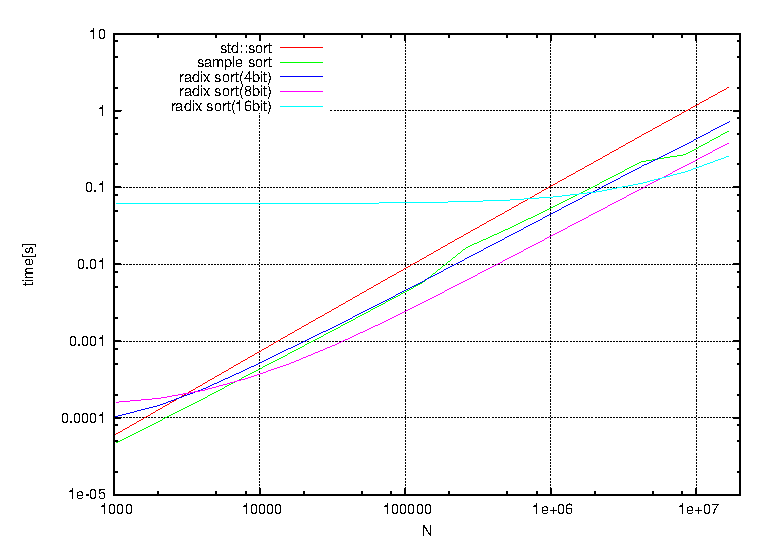
\includegraphics[width=15cm]{fig/sorting_time.eps}
  \end{center}
  \caption{ソート時間の比較}
  \label{fig:sorting_time}
\end{figure}

\newpage

次にツリー構造をトップからレベル毎に作っていく。ツリーのセルを作るのに
はバイナリーサーチを使う。粒子数が少なくなってきたらリニアサーチを使っ
た方が良いかもしれないが実装していない。子セルをアロケートする場所を決
めるのにprefix sumを使っているが、スレッド並列化はしていない。以下の関
数により、ツリー構造が作られる。この関数はモートンソート前に呼んではな
らない。

\begin{screen}
\begin{verbatim}
void linkCellLocalTreeOnly();
\end{verbatim}
\end{screen}

モーメントの計算は下のレベルから順に行う。ツリーセルはレベル毎に連続で
メモリー上に並んでいるので、各レベルでスレッド並列で行う。モーメントの
計算は次の関数で行う。

\begin{screen}
\begin{verbatim}
void calcMomentLocalTreeOnly();
\end{verbatim}
\end{screen}


図\ref{fig:makeLT}は京で8スレッド使った時にローカルツリー作りにかかる時
間。

\begin{figure}[h]
  \begin{center}
    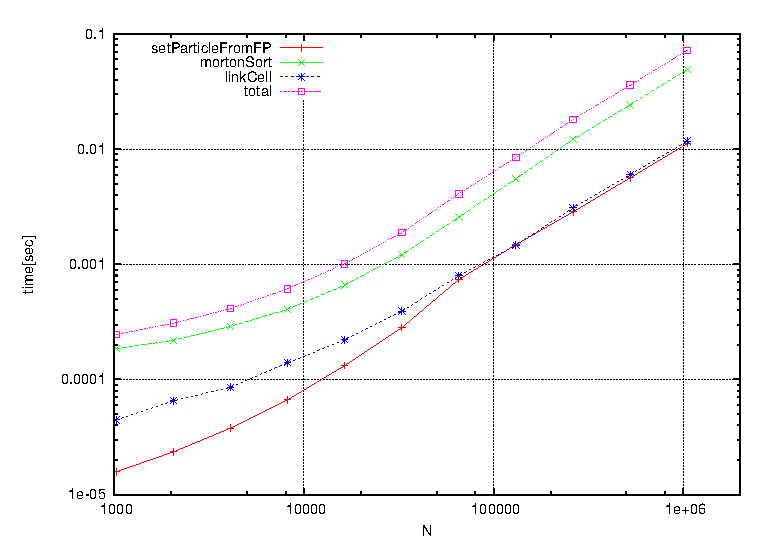
\includegraphics[width=15cm]{fig/timeingLT.eps}
  \end{center}
  \caption{ローカルツリー構築}
  \label{fig:makeLT}
\end{figure}

\newpage

図\ref{fig:makeLT}はXeon(2.93GHz, Nehalem)で6スレッド使った時にローカル
ツリー作りにかかる時間。モーメント計算は重心の計算のみ。

\begin{figure}[h]
  \begin{center}
    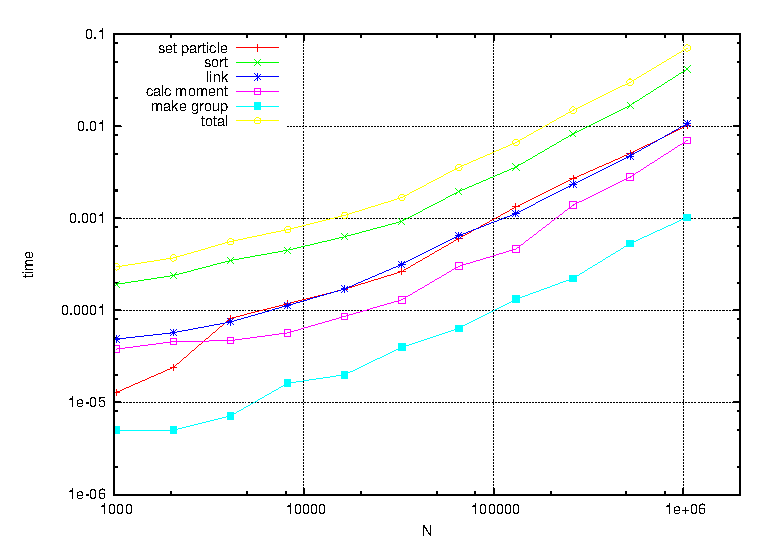
\includegraphics[width=15cm]{fig/timeingLT_xeon.eps}
  \end{center}
  \caption{ローカルツリー構築}
  \label{fig:makeLT}
\end{figure}

\newpage

{\bf radix sort クラス}

radix sort クラスは以下の様になっている。

\begin{lstlisting}[caption=RadixSort]
namespace ParticleSimulator{
    template<class T, int NBIT=8>
    class RadixSort{
    private:
        int n_thread_;
        int n_bucket_;
        T mask_;
        int ** bucket_size_;
        int ** prefix_sum_;
    public:
        RadixSort();
        template<class Tobj>
        void lsdSort(Tobj * & val,
                     Tobj * & val_buf,
                     const int first,
                     const int last);
    };
}
\end{lstlisting}

注意として、このクラスはunsigned型の整数のみに対応している。また、メソッ
ド{\tt lsdSort}でOpenMPを使っている。

クラステンプレートパラメータは最初がソートする対象の型(U64)、
{\tt NBIT}はradixのビット数でデフォルトは8bit。コンストラクタにより、メ
ンバの領域や値が代入される。

%%%%%%%%%%%%%%%
\begin{screen}
\begin{verbatim}
template<class Tobj>
void lsdSort(Tobj * & val,
             Tobj * & val_buf,
             const int first,
             const int last);

\end{verbatim}
\end{screen}

\begin{itemize}

\item{{\bf 引数}}

{\tt val}: 入力、出力。

{\tt val\_buf}: 入力。

{\tt first}: 入力。

{\tt last}: 入力。

\item{{\bf 返り値}}

なし。

\item{{\bf 機能}}

{\tt val}のメソッド{\tt getKey()}により返される値の順に{\tt val}をソー
トする。{\tt val\_buf}は{\tt val}と同じ型、サイズの配列でソートする時の
バッファー領域として使う。{\tt first}はソートする配列の領域の最初のイン
デックス、{\tt last}はソートする配列の領域の最後のインデックス。内部で
はOpenMPを用いて並列化されている。

\end{itemize}

使い方はまずオブジェクトを作り、メソッド{\tt lsdSort()}を呼び出す。
\begin{lstlisting}[caption=RadixSortの例]

    PS::TreeParticle * data = new TreeParticle[n_size];
    PS::TreeParticle * data_buf = new TreeParticle[n_size];
    for(int j=0; j<n_size; j++){
        data[j].setKey(PS::U64(abs(rand()))<<32 | PS::U64(abs(rand())));
    }
    PS::RadixSort<PS::U64, 8> RS;
    RS.lsdSort(data, data_buf, 0, n_size-1);

\end{lstlisting}

\subsubsubsection{相互作用計算に必要な粒子の交換}

前提として、全プロセスのドメインの座標を全プロセスが持っている(領域分割
時に全座標を放送する)。

\subsubsubsubsection{開放境界、長距離力カットオフなし}

他ドメインに対して自プロセスのツリーをたどり、他ドメインが力を計算する
のに十分なEPJ、SPJをそれぞれ、{\tt ep\_j\_send\_}、{\tt sp\_j\_send\_}
に格納する。またその個数を{\tt n\_ep\_j\_send\_[]}、{\tt
n\_sp\_j\_send\_[]}に格納する。配列のインデックスはプロセス番号と対応さ
せること。まず、{\tt n\_ep\_j\_send\_[]}、{\tt n\_sp\_j\_send\_[]}を
Alltoallし、受信した値を{\tt n\_ep\_j\_recv\_[]}、{\tt
n\_sp\_j\_recv\_[]}に格納する。次にAlltoallvを使い{\tt ep\_j\_send\_}、
{\tt sp\_j\_send\_}を送り、受信した値を{\tt ep\_j\_recv\_}、{\tt
sp\_j\_recv\_}に格納する。

\subsubsubsubsection{開放境界、長距離力カットオフあり}

自ドメインと他ドメインの距離を測り、カットオフ半径より短い場合はローカ
ルツリーをたどる。辿り方はほとんど”長距離力カットオフなし”の場合と同
じだか、ツリーセルと他ドメインの距離がカットオフ長より長い場合はそのセ
ルを辿る必要は無い。通信は粒子数を送る所は”長距離力カットオフなし”の
場合と同じだが、粒子は全てのノードに送るわけではないのでAlltoallvを使わ
ずにIsend, Irecvで送る。

\subsubsubsubsection{開放境界、短距離力散乱モード}

%他プロセスのツリールートセルの内側境界(ドメインでも良い)に対して自プロ
%セスのツリーを辿る。この時ツリーの外側境界を使って、

他プロセスのドメインに対して自プロセスのツリーを辿る。この時ツリーの外
側境界を使って、他プロセスのドメインとの距離を測る。通信パターンは"開放
境界、長距離力カットオフあり"の場合と同じ。


\subsubsubsubsection{開放境界、短距離力収集モード}

最初に、ツリールートセルの外側境界の座標をAllgatherする。他プロセスのツ
リールートセルの外側境界に対して自プロセスのツリーを辿る。この時ツリー
の内側境界を使って、他プロセスのドメインとの距離を測る。

上記の方法だと、例えばプロセス内の粒子にカットオフ半径のばらつきがあっ
た場合など、通信量が非常に増えてしまう場合も考えられる。そこで、以下の
様な方法も考えられる。まず、”短距離力散乱モード”と同様の方法で、粒子
を送る(Alltoallで粒子数を送り、Isend,IredvでEPJを送る)。次に送られて来
た粒子のカットオフ半径内に入り、かつ送られて来た粒子の送信元プロセスの
ルートセルのドメインとの距離がそのカットオフ半径より長い粒子(「送信元」
プロセスには送られていない粒子)を{\tt ep\_j\_send\_}に格納する。

%送信する粒子が重複しないようにソート等を行う。粒子を送ったプロセスから
%しか粒子は送られてこないので、粒子数、EPJをIsend,Irecvで通信する。この
%ようにすると送られて来た粒子は散乱モードと収集モードの和集合を含むので
%十分である。




\subsubsubsubsection{開放境界、短距離力対称モード}

最初に、ツリールートセルの外側境界の座標をAllgatherする。他プロセスのツ
リールートセルの外側境界に対して自プロセスのツリーを辿る。この時ツリー
の外側境界を使って、他プロセスの外側境界との距離を測る。

収集モードの場合で述べた2段階通信の方法も考えられる。

%ルートセルの外側境界とが重なっているかを判定する。
%重なっている場合はツリーを辿り、重なりのあるリーフセルの粒子と他プロセ
%スの外側境界との距離がその粒子のカットオフ半径より短い場合はその粒子を
%送る。

%集積モードの場合と同様に、カットオフ半径にばらつきがあると通信量が増え
%てしまう可能性がある。そこで集積モードの場合と同様に2段階で通信する方
%法も考えられる。まず、”短距離力散乱モード”と同様の方法で、粒子を送る。
%次に送られて来た粒子のカットオフ半径内に入り、かつ送られて来た粒子の送
%信元プロセスのルートセルの内側境界(もしくはドメイン)との距離がそのカッ
%トオフ半径より長い粒子(「送信元」プロセスには送られていない粒子)を送信
%する。

\subsubsubsubsection{開放境界、短距離力固定モード}

短距離力散乱モードと同じ実装を行う。

\subsubsubsubsection{直方体周期境界、長距離力カットオフあり}

\subsubsubsubsection{直方体周期境界、短距離力散乱モード}

\subsubsubsubsection{直方体周期境界、短距離力収集モード}

\subsubsubsubsection{直方体周期境界、短距離力対称モード}

\subsubsubsubsection{直方体周期境界、短距離力固定モード}

\subsubsubsection{グローバルツリーの作成}

\subsubsubsubsection{開放境界条件}

{\tt ep\_j\_recv\_},{\tt sp\_j\_recv\_}から{\tt tp\_glb\_}を作る。この
際TPの{\tt adr\_ptcl\_}は{\tt ep\_j\_recv\_},{\tt sp\_j\_recv\_}の配列
のインデックスを入れるが、EPJとSPJを区別するためにSPJのMSBは1にする。ツ
リー構築はローカルツリーと同様。最初はモートーンソートを作ってからのツ
リー構築を実装する。LETが少ない場合は挿入の方が速いかもしれない。

\subsubsubsubsection{直方体周期境界条件}


\subsubsubsection{i粒子グループ構築}

{\tt PS}ではいくつかのi粒子群に対してツリーを辿るので、相互作用の計算の
前にi粒子グループの構築を行う。これは、ローカルツリーの構造を使うだけな
ので、ローカルツリー構築以降、相互作用計算の前ならどこでも行う事が出来
るので、LET交換にオーバーラップさせることも出来る。ただし、この計算コス
トは軽いのであまり意味がないかもしれない。

以下にi粒子群を表すクラスを示す。

\begin{lstlisting}[caption=IPGroup]
namespace ParticleSimulator{
    template<int Tsmode>
    class IPGroup{
    public:
        F32ort vertex_;
        S32 adr_ptcl_;
        S32 n_ptcl_;
        template<class Ttc> void copyFromTC(const Ttc & tc);
    };
\end{lstlisting}

{\tt vertex\_}はi粒子グループを囲む直方体の座標で、力の種類によって表現
するものが異なる。力の種類はテンプレートパラメータとして与えられる。短
距離力散乱モードでは内側境界、短距離力収集モードと短距離力対称モードと
短距離力固定長モードでは外側境界を使う。長距離力では内側境界を使うと計
算量がツリーセルがスパースなところでは計算量が減るが絶対必要というわけ
ではないので、長距離量の場合の実装をどうするかは未定。{\tt
adr\_ptcl\_}は{\tt ep\_i\_}のインデクスで、{\tt n\_ptcl\_}はそのi粒子群
の個数である。{\tt ep\_i\_}は順番に並んでいるのでインデックスと粒子数だ
けあれば計算可能である。

以下の関数により、i粒子グループを作る。

\begin{screen}
\begin{verbatim}
void makeIPGroup();
\end{verbatim}
\end{screen}

\subsubsubsection{相互作用の計算}



\subsubsubsection{相互作用の書込}


\subsubsubsection{近傍粒子探査}

{\tt SEARCH\_MODE}が{\tt LONG_SCATTER}、{\tt LONG_CUTOFF_SCATTER}、
{\tt LONG_SYMMETRY}、{\tt LONG_CUTOFF_SYMMETRY}の場合には以下に述べる
近傍粒子探査用の関数が使える。
\redtext{{\tt LONG_SYMMETRY}、{\tt LONG_CUTOFF_SYMMETRY}は未実装}。

%\subsubsection{相互作用ツリークラス}


\subsection{拡張モジュール詳細}
\label{sec:detail_option}


%%%%%%%%%%%%%%%%%%%%%%%%%%%%%%%%%%%%%%%%%%%%%%
\subsubsection{Particle Meshクラス}
\label{sec:detail_option_particle_mesh}

この節では、Particle Meshクラスの詳細記述を行う。Particle Meshクラスを
以下のように記述した。

関数{\tt calcForceAllAndWriteBack}はParticle Meshによる力を全粒子に対し
て計算し、その計算結果を書き込むことまで行う。その他の関数が必要となる
のは、複数種類の粒子を扱う場合だけである。

\begin{lstlisting}[caption=ParticleMesh]
namespace ParticleSimulator {
    namespace ParticleMesh {
        class ParticleMesh{
        public:
            template<class Tpsys,
                     class Tdinfo>
            void calcForceAllAndWriteBack(const Tpsys & psys,
                                          const Tdinfo & dinfo);
            template<class Tdinfo>
            void setDomainInfoParticleMesh(const Tdinfo & dinfo);
            template<class Tpsys>
            void setParticleParticleMesh(const Tpsys & psys,
                                         const bool clear=true); 
            void calcMeshForceOnly();
            F32vec getForce(F32vec pos);
        }
    namespace PM = ParticleMesh;
}
namespace PS = ParticleSimulator;
\end{lstlisting}

粒子クラスに粒子質量のゲッターとなるメンバ関数が必要。質量のメンバ変数
が{\tt mass}である場合は、以下のように書く。
\begin{screen}
\begin{verbatim}
void getChargeParticleMesh() {
    return this->mass;
}
\end{verbatim}
\end{screen}

\subsubsubsection{全粒子への力を計算する関数}

\begin{screen}
\begin{verbatim}
template<class Tpsys,
         class Tdinfo>
void PS::PM::calcForceAllAndWriteBack(const Tpsys & psys,
                                      const Tdinfo & dinfo);
\end{verbatim}
\end{screen}

上の関数で、全粒子への力を計算し、計算結果を粒子群クラスへ格納する。
{\tt psys}は力を計算すべき粒子群クラス、{\tt dinfo}は領域クラスである。

計算結果を粒子群クラスへ格納するためのセッターが必要である。粒子クラス
にメンバ関数{\tt copyFromForceParticleMesh(const PS::F32vec \& force)}
を設定する必要がある。もし、Particle Meshによる力のメンバ変数が{\tt
  PS::F32vec apm}であるなら、以下のように記述する。
\begin{screen}
\begin{verbatim}
void copyFromForceParticleMesh(const PS::F32vec & force) {
    this->apm = force;
}
\end{verbatim}
\end{screen}
また、Particle--particleの力(メンバ変数を{\tt acc}とする)にそのまま足し
こむ場合、以下のように記述する。
\begin{screen}
\begin{verbatim}
void copyFromForceParticleMesh(const PS::F32vec & force) {
    this->apc += force;
}
\end{verbatim}
\end{screen}
この関数を使わない場合は、このセッターを用意する必要はない。

この関数は、全プロセスで呼びだす必要がある。

\subsubsubsection{領域クラスをセットする関数}

\begin{screen}
\begin{verbatim}
template<class Tdinfo>
void PS::PM::setDomainInfoParticleMesh(const Tdinfo & dinfo);
\end{verbatim}
\end{screen}

上の関数で、このクラスに領域クラスの情報を与える。引数の{\tt dinfo}は領
域クラスである。

この関数は、全プロセスで呼びだす必要がある。

\subsubsubsection{粒子情報をセットする関数}

\begin{screen}
\begin{verbatim}
template<class Tpsys>
void PS::PM::setParticleParticleMesh(const Tpsys & psys,
                                     const bool clear=true);
\end{verbatim}
\end{screen}

上の関数で、このクラスに粒子群クラスの情報を与える。第1引数の{\tt }は
粒子群クラスである。第2引数はすでに与えられた粒子群クラスの情報をクリ
アするかどうかを決める。{\tt true}のときはクリアし、{\tt false}のときは
クリアしない。

この関数は、全プロセスで呼びだす必要がある。

\subsubsubsection{メッシュ上の力を計算する関数}

\begin{screen}
\begin{verbatim}
void PS::PM::calcMeshForceOnly();
\end{verbatim}
\end{screen}

メッシュ上の力を計算する。

この関数は、全プロセスで呼び出す必要がある。

\subsubsubsection{1つの粒子への力を計算する関数}

\begin{screen}
\begin{verbatim}
PS::F32vec PS::PM::getForce(PS::F32vec pos);
\end{verbatim}
\end{screen}

1つの粒子への力を計算し、その計算結果を返す関数である。引数{\tt pos}は
力を計算したい粒子の位置である。返す値は計算結果の力である。

\subsubsubsection{Particle Meshクラスの使い方}

Particle Meshクラスを使うには以下の4つのことを行う必要がある。
\begin{enumerate}
\item MPIとFFTWのインストール
\item Particle Meshクラスのコンパイル
\item Particle Meshクラスを使ったFDPSコードの記述
\item FDPSコードのコンパイル
\end{enumerate}
以下、詳細に記述する。

\subsubsubsubsection{MPIとFFTWのインストール}

ぐっどらっく

\subsubsubsubsection{Particle Meshクラスのコンパイル}

以下のように行う。ディレクトリ{\tt src\_parallel}の下のディレクトリ
{\tt particle\_mesh}のMakefileを適切に編集してmakeする。編集すべきこと
は以下の2点である。
\begin{itemize}
\item {\tt INCLUDE\_FFTW}にFFTWのヘッダファイルがあるディレクトリを記述
  する
\item param\_fdps.hの中のSIZE\_OF\_MESH (1次元方向のメッシュの数)を設定。
推奨値は $N^{1/3}/2$($N$は粒子数)。
\end{itemize}
うまく行けば、同じディレクトリにライブラリ{\tt libpm.a}とヘッダファイル
{\tt particle\_mesh.hpp}ができている。

\subsubsubsubsection{FDPSコードを記述}

以下のように行う。
\begin{itemize}
\item 上でできたヘッダファイルをincludeする
\item PMを計算したい粒子クラスに以下のメソッドを加える
     \begin{itemize}
     \item void copyFromForceParticleMesh(const PS::F32vec \& force)。こ
     の中でforceを好きなメンバ変数にセットする。
     \item PS::F64 getChargeParticleMesh()。この中で質量を返す。
     \end{itemize}
\item このクラスのインスタンスを生成するときに、{\tt PS::PM::ParticleMesh}と
する
\end{itemize}

\subsubsubsubsection{FDPSコードのコンパイル}

上で記述したFDPSコードをコンパイルするには以下のことを行う必要がある。
\begin{itemize}
\item ヘッダファイル{\tt particle\_mesh.hpp}のあるディレクトリを記述す
  ること
\item ライブラリ{\tt libpm.a}とのリンク
\item FFTWのヘッダファイルがあるディレクトリを記述すること
\item FFTWのライブラリとのリンク
\end{itemize}

%\subsubsection{Particle Meshクラス}
